\chapter{Conclusion and Perspectives}\label{conclusion}

\section{Contributions}

The purpose of the thesis was to propose solutions to better use medical images in order to provide a better characterization of the liver tumors. We successfully presented results proving the ability of deep learning to accurately delineate the liver and its tumors on dynamic CECT images. Moreover, we presented preliminary results proving the ability of automatically extracted deep multiphase imaging features to predict the histological grade of HCCs.\\
After describing the potential causes that can lead to the different
types of liver cancer, we motivated our choice to mainly focus on
hepatocellular carcinoma (\ac{hcc}).
This primary cancer type, which is the most frequent one, was described
through its origin, the way it is usually diagnosed, classified and
treated.
The different steps transforming healthy hepatic cells to cancerous ones
have been described, along with the analysis of the physiological
changes often caused by this process.
To better characterize the liver tumors, we have decided to rely on
medical images solely, through a quantitative and objective analysis.
Regarding the modality choice, we retained the computed tomography
because it currently corresponds, with \ac{mri}, to the most widely used modality 
for a non-invasive assessment of the disease.
CT was chosen over \ac{mri} mainly since it is usually the first choice for
less-specialized centers, and because it can be more easily interpreted
than \ac{mri}. With our medical studies review, we showed that the use of
dynamic temporal images is a prerequisite to conduct an imaging based liver cancer
study.

In the present work, we presented the two paradigms allowing the computer
assisted analysis of medical images, either with engineered features, or
thanks to deep-learning. One of the key aspects of medical images
analysis being the segment, we compared the different semantic
segmentation architectures, and evaluated the benefit brought by
multiphase images which was most of the time neglected by previously
existing studies. Then we extracted relevant features from our semantic
segmentation architecture to tackle the prediction of the histological
grade. Each step of our research work required imaging databases
precisely annotated by experts in association with researchers to
improve their applicability.

In the clinical practice, images are usually analyzed by the experts
with the naked eye, but the technological advancements allowed the
creation of computer assisted diagnosis tools (CADs), where a few number
of imaging features were initially used to differentiate benign and
malignant lesions.
A new technology called radiomics has been developed to compute a higher
number of features but it took a long time before this technology was
applied to the liver, especially because of the scarcity of publicly
available datasets.
We provided a detailed description of the radiomics pipeline, 
based on a manual segmentation of the \ac{roi}, followed by the extraction of
a high number of engineered quantitative features, thus being called
\emph{\ac{hcr}} (Hand-Crafted Radiomics).\\
We presented our review, where a total of 15 \emph{\ac{hcr}} studies
performed on \ac{hcc} patients have been analyzed.
We evaluated them against the radiomics quality score (\emph{RQS})
which has been developed to assess the robustness and the
reproducibility of radiomics studies.
We pointed out the lack of reproducibility of the studies, with a mean
\emph{RQS} of 8.73 +/- 5.57 points out of a possible maximum value of 36
points.\\
Several important criteria were found as being ignored by the majority
of the studies, such as a prospective design, the use of open-sourced
data, the evaluation of the prediction on a validation dataset, or the
extraction of features at multiple timepoints.

The emergence of deep learning has changed the way a lot of imaging
related problems are comprehended.
The radiomics field has been also impacted by this novel set of
algorithms, and a new paradigm called \emph{\ac{dlr}} (Deep-Learning
Radiomics) has been initiated, where one or several steps of the
radiomics pipeline are performed by deep learning algorithms.\\
We believe that the key part of the radiomics pipeline lies in the
segmentation of the \ac{roi}. This step has been found to suffer from a high
inter- and intra-observer variability, thus having consequences for the
accuracy of the final prediction. \\
We reviewed the different studies using deep learning architectures to
perform automatic segmentation of the liver and its tumors. We extracted
the common key settings shared by the majority of them, such as the
cascaded architecture or the use of fully convolutional networks.
However, we realized the lack of studies presenting results obtained
from multiphase images, which has been a key element in our work. \\
We performed the automatic segmentation of an internal dataset composed
of 104 sparse biphasic liver slices obtained from patients suffering
from \ac{hcc} (images available before the injection of contrast medium:
Non-Enhanced \ac{ct}, and at both arterial and portal venous phases).
Considering how challenging the segmentation of liver tissues is, the
amount of data, and the success of such an architecture, we decided to
train several specialized networks in a cascaded way.\\
When evaluating the performances of each specialized network, we
validated the hypothesis that the use of multiphase information allows a
better accuracy than single phased based networks for each task,
with significant difference obtained for the segmentation of the liver
(mean \ac{dsc} of $ 89.9 \pm 15.6 $ for the multiphase network \emph{vs} $ 89.5 \pm
13.2 $ for the best single phase network) and the active part of the
lesions (mean \ac{dsc} of $ 75.5 \pm 17.4 $ \emph{vs} $ 71.6 \pm 20.7 $).\\
Regarding single phase networks, the \emph{\ac{pv}} phase was the one
allowing the most accurate segmentation, with significant difference vs
\emph{\ac{ar}} and \emph{\ac{nect}} for the segmentation of the parenchyma (mean
\ac{dsc} of $ 88.7 \pm 15.4 $) , the lesion (mean \ac{dsc} of $ 87.8 \pm 9.7 $), and both the
necrotic (mean \ac{dsc} $ 77.8 \pm 12.4 $) and the active (mean \ac{dsc} of $ 71.6 \pm 20.7 $)
part of the lesion. \\
We validated the hypothesis that several specialized networks combined
in a cascaded architecture perform better than a single network
addressing all the tasks simultaneously (obtained mean slice-wise \ac{dsc} of
$ 90.5 \pm 13.2 $ for the parenchyma, $ 75.8 \pm 15.1 $ for the necrosis and $ 59.6 \pm
22.5 $ for the active part of the tumor when using the cascaded
architecture with the liver \ac{gt} mask as input).\\
In a fully automatic manner (without using the liver \ac{gt} mask), we were
able to reach promising results regarding the size of the dataset, with
a mean slice-wise \ac{dsc} of $ 78.3 \pm 22.1 $ for the parenchyma, $ 50.6 \pm 24.6 $ for
the active tumor and $ 68.1 \pm 23.2 $ for the necrotic part of the tumor.\\
We were also able to automatically compute the necrosis rate of the
tumors, with a mean error of 15.9\% when compared with the experts
obtained rates. This prediction is accurate enough to consider the
predicted necrosis rate when evaluating the treatment outcomes. \\
To overcome the limited size of multiphase datasets, we defined a
strategy to ``augment'' the weakly annotated or non-annotated available
datasets.
With a robust registration algorithm and our cascaded architecture where
specialized networks are trained on a sufficient amount of data, we were
able to perform the semantic segmentation of liver and its tumors on
unseen cases.
We validated this assumption by performing the segmentation of TCIA
tumors, and obtained a mean patient-wise \ac{dsc} of $ 73.2 \pm 20.6 $.\\
To predict the histological grade, we proved that features learned by
our multiphase semantic segmentation network are relevant to perform
this task.
We predicted the grade for central tumor slices, and after a CV
training, we correctly predicted 74\% of them. When considering the
patient histological grade as being the most frequent one in the central
tumor slices, we were able to correctly classify 15 patients over the 18
of the dataset.\\
As a conclusion, our research work is the first to propose a fully
automatic \emph{\ac{dlr}} pipeline with multiphase images as input. Our
strategy is dedicated to small databases where the entire annotations
are often not available but the same workflow can be applied for larger
datasets. Our \emph{\ac{dlr}} architecture was dedicated, in this research
work, to the prediction of the histological grade of \ac{hcc} patients, but
our strategy can be extended to other characteristics of \ac{hcc} or other
types of liver cancers.\\
Regarding the lack of publicly available datasets, we encourage the
creation of an open 3D \ac{cect} dataset containing liver volumes of both
healthy and diseased patients with precise and complete pathological
information, and expert delineations of liver, hepatic vessels and
lesions for each phase.


\section{Perspectives}

Several axes of improvement can be considered regarding our research work.
We will discuss potential improvements to bring to the 
semantic segmentation of liver tumors, before raising issues regarding
the current standards for dynamic \ac{cect} acquisition and their impact to 
future multiphasic \ac{ct}-based radiomics studies.
Finally we present ways to incorporate our work in other \ac{dlr}-liver related 
studies, by encouraging for the creation of open and precisely 
annotated \ac{cect} datasets.
%When performing a hand-crafted or a deep radiomics study, we still
%believe that the key part will be the area selection preceding the
%computation of the radiomics features.

\subsection{Semantic Segmentation}

As discussed before, the \ac{hcr} paradigm often requires manual experts
segmentations, and several studies already discussed the inter- and
intra-observer variability present among the obtained delineations. This
variability is translated in the quality of the retained features, which
tend not to be robust enough when evaluating the predictive 
strength of the model.\\
The \ac{dlr} paradigm allows one or multiple steps of the radiomics pipeline to be implemented with deep learning approaches. We decided to focus on the segmentation step and performed it automatically thanks to deep neural networks, thus reducing the number of potential biases. The automatic segmentation, as
performed in our research work, however requires a high number of
training cases to offer a realistic delineation of the targeted tissues.\\
In the case of liver tumors, a cascaded architecture stacking a first
network responsible for the segmentation of the liver and a second
dedicated only to detect the tumor within the obtained liver mask is
currently the method allowing to obtain the most accurate results.
State-of-the-art liver segmentation methods currently allow us to reach
annotations similar to those obtained by the experts with mean \ac{dsc} often
above 0.95-0.96. We believe that there is no real need to improve the
liver segmentation in the future, and that more interest needs to be
shown in tumor and other liver tissues segmentation.

Regarding the segmentation of liver tumors, current state-of-the-art
results were obtained thanks to post-processing steps such as false
positives (\ac{fp}) filtering method to reduce the number of
objects misclassified as lesions.
It might be that current semantic segmentation architectures still lack the
ability to discriminate between real lesions and other areas of the liver sharing the
same textural properties such as regions close to the vessels as
illustrated in the figure \ref{fig:image5}.



\begin{figure}[th!]
\centering
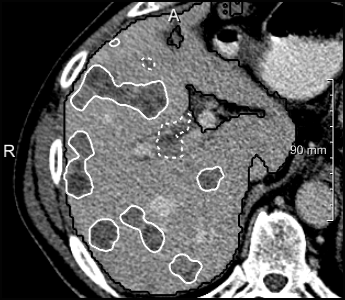
\includegraphics[width=0.5\linewidth]{../Perspectives/images/chlebus}
\caption{Tumor candidates marked with a dashed white line were classified as false positives, as described by \textbf{Chelbus et al. \cite{Chlebus2018}}.}
\label{fig:image5}
\end{figure}

This low recall might be explained by the poor quality of the
currently available segmentation datasets. Liver annotations often
contain non-hepatic areas (such as air most of the time) or
imperfections close to the organ borders.
When performing the automatic liver segmentation, the deep neural
networks will most of the time be able to avoid these regions. However,
in case they are integrated in the liver mask, they will often be
misclassified as tumors by the second network in the cascade
(responsible for the tumor segmentation).

To overcome this issue, publicly available datasets such as the
\lmttfont{LIST-dB} need to be properly resegmented. They usually only contain
annotations for the parenchyma and/or the tumors, but a third class (or
more) could be incorporated, in order to consider tissues belonging to none of
these groups such as the cysts or the blood vessels.\\
As explained in the section  \ref{subsection:StateOfTheArtDlImplementations}, current state-of-the-art tumor
segmentation results are often obtained with 2D or 2.5D networks, but
the post-processings steps usually help to improve the obtained accuracy
(via 3D CRF or even simple morphological operations). Several studies
implemented a U-Net like architecture, where the information is
compressed before being decoding to obtain the final segmentation map.
One of the key concepts in these architectures is the propagation of
features learned in the earlier layers later in the network, either
thanks to skip-connections, residual units or even densely connected
layers. Another way to perform the segmentation could be by implementing a
multi-scale pyramidal architecture where tumor-related features can be
learned directly from the raw images at multiple scales instead of being
learned from previously computed features, which is often the case in
the aforementioned architectures.\\
It might also be interesting to perform the segmentation with a full 3D
architecture. Some studies already investigated this solution \cite{Dou2016}, 
but they could not yet outperform state-of-the-art results. \\
Some other concepts could be incorporated in future architectures. Jin et
al. \cite{Jin2018} for example proposed a network that integrated both U-Net and
attention residual mechanism to proceed the segmentation of both the
liver and the lesions. The residual attention mechanism has been
introduced in 2017 by Wang et al. \cite{Wang2017} to perform image
classification, with the idea that the attention mechanism can help the
network focusing on specific parts of the image. The study from Jin et
al. was the first to use the attention mechanism for
semantic segmentation purposes. On the hidden test set of LITS, they
outperformed a lot of 2D-based methods, but were still far from the
top-ranked teams. However, new paradigms such as the self-attention
mechanism, in combination with state-of-the-art 2D and 3D architectures
are certainly an avenue for the improvement of the automatic liver and
tumors segmentation tasks \cite{Chen2019}.

\subsection{Dynamic contrast-enhanced images}

In our research work, the key element is the extraction of features
from dynamic contrast-enhanced images. However, it has been very
difficult to collect dynamic \ac{cect} based images, since only a few
publicly available datasets contain this type of volume. \\
There is a huge room for improvement regarding this specific type of
dataset. It has been mentioned in the chapter \ref{liverCancer}, that the
use of images obtained after the injection of contrast medium largely
improves the visual and the automatic quality of the diagnosis.
Nonetheless, we realized that multiphasic images could be better used in
either the semantic segmentation and/or the radiomics field.\\
The first issue is related to the acquisition protocol required to
obtain this type of images. Most of the time, the different retained
phases, namely arterial, portal venous or delayed phases are acquired
following either visual inspection of the radiologists \footnote{The arterial phase is sometimes acquired
with the help of a bolus tracking technique}, or after a specific
duration following the injection moment that can differ from one study
to the other. Another criteria to consider is the physiological
characteristics of the patient such as its weight that will determine
how the contrast medium is diffused through the liver.

When dealing with multiphase databases, we believe that these key
elements need to be considered, at least the moment of injection and/or
the duration between the injection and the acquisition.  
%since the weight
%of the patient can be inferred from the liver volume (which can be
%predicted thanks to semantic segmentation).
Currently, only the DICOM
format allows the addition of such metadata (it is only possible to record 
the exact acquisition moment but not the injection moment) 
but they are barely reported and
are often left to default values.\\
Obtaining such data seems really challenging, hence, some techniques
need to be implemented to deal with current multiphase images. 
For example, we believe that a ``phase correction system'', responsible for 
the normalization of images belonging to the same phase, could be
implemented . The automatic detection of the amount of contrast medium still in
the liver could also help to predict the exact duration between the
injection of the contrast medium and the acquisition.

In our research work, we have decided to implement an histogram
specification algorithm to ``normalize'' images from a given phase. The
first step requires to compute a mean histogram per phase (which requires to
have a sufficient amount of \ac{ct} images correctly labeled), before
transforming the volumes of a given patient to match the obtained mean
histogram, as depicted in the figure \ref{fig:specif}.

\begin{figure}[ht!]
\centering
\begin{minipage}{0.5\linewidth}
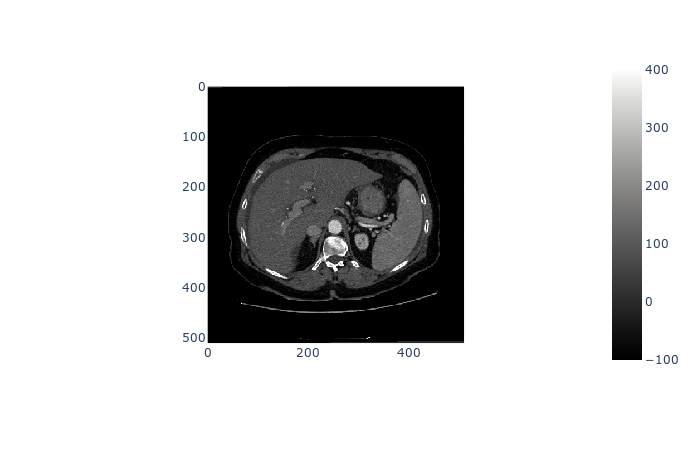
\includegraphics[width=\linewidth]{../Perspectives/images/image3.png}
\end{minipage}
\begin{minipage}{0.5\linewidth}
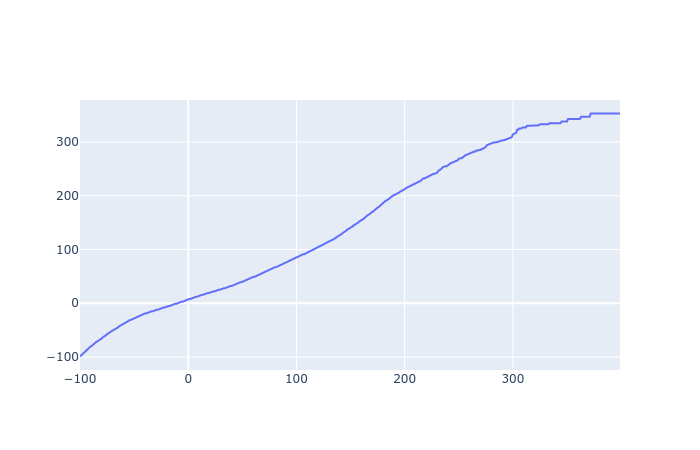
\includegraphics[width=\linewidth]{../Perspectives/images/image1.png}
\end{minipage}
\begin{minipage}{0.5\linewidth}
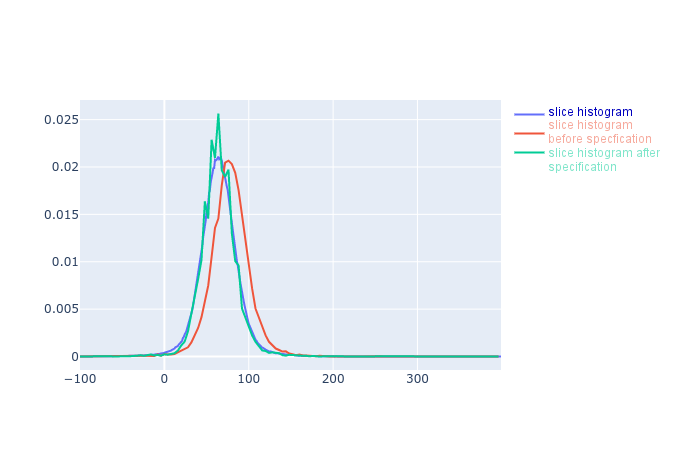
\includegraphics[width=\linewidth]{../Perspectives/images/image2_modified.png}
\end{minipage}
\begin{minipage}{0.5\linewidth}
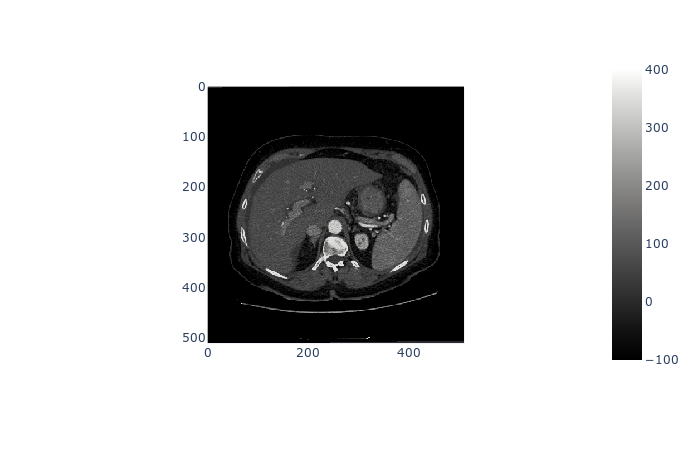
\includegraphics[width=\linewidth]{../Perspectives/images/image4.png}
\end{minipage}
\caption{Histogram specification experiment conducted to normalize images from the same phase, top row: slice before histogram specification; second row: mapping function for the chosen range [-100, 400]; third row: representation of the mean phase histogram, the current slice histogram and the transformed one after application of histogram specification; bottom row: slice after histogram specification.}
\label{fig:specif}
\end{figure}

In the case of multiphase images, the expert performing the segmentation
will usually try to obtain only one segmentation volume shared by all the 
registered volumes. This representation might be coherent for the liver mask, 
but we believe that it needs to be modified for internal liver tissues. 
The lesions, for example, will have a different behavior from one phase to the other
(hypo- or hyper-dense tumors for example), consequently, one segmentation per phase should
be performed. This might potentially help the deep neural
networks to better understand the dynamic of the lesions, and also
address the problem of small mis-registration when only one ground truth
segmentation map is shared by all the available phases images.

One long-term objective could be to create, with the help of
radiological experts, a dataset containing registered multiphase \ac{ct}
volumes with expert annotations performed following the aforementioned
protocol.

\subsection{Deep Radiomics}

Regarding our \ac{dlr} study, we believe that the prediction of the
histological grade can be improved. \\
As an example we advocate for a grade prediction at a finer
scale, but it will require to know the exact position of the extracted
sample, or to obtain a map of the heterogeneous regions after surgical
removal of liver tissues through liver resection or liver transplant for
example.\\
In our research work we investigated a patch-wise prediction of the
histological grade but the results were not as promising as those
obtained through our slice-wise approach, especially because our
patch-wise semantic segmentation network needs to be improved.

We are considering the relevant imaging features as being the
ones extracted from the bottleneck part of our U-Net network but other
types of auto-encoders could be investigated to better
extract the relevant information from the raw images, or from the
retained features. We could have also incorporate clinical
data (\ac{afp} (Alpha-FetoProtein) levels, age, \ldots{}) in our pipeline, however such data are
often difficult to retrieve, and challenging to combine with imaging
features, consequently, we decided to focus only on images in the
current work.\\
It is worth also noting that the current registration steps still suffers from limitation
essentially because it performed using the predicted liver masks as registrations masks. However, the automatic liver delineations is not perfect, and therefore this can result in slightly misregistered volumes. Therefore, we advocate an incorporation of an automatic deep learning based registration step in our \ac{dlr} pipeline, or a workflow requiring no registration at all (for example by considering features learned in each phase separately and combining them for the grade prediction).\\
If more interest is shown in the future towards the prediction
histological grade, we believe that the existing grading systems have to
be standardized by considering more criteria than just the worst or the
most frequent grade present in the histological slices, which is
currently the case.\\
Our \ac{dlr} architecture obtained promising results for the prediction of
the histological grade, but we believe that the same architecture can be
adapted to focus on other tasks, such as the prediction of
recurrence after treatment using longitudinal studies.
